\documentclass[12pt,a4paper]{report}
\usepackage[utf8]{inputenc}
\usepackage[czech]{babel}
\usepackage{amsmath,amssymb}
\usepackage[top=3.5cm, bottom=3.5cm, left=3.5cm, right=2.5cm]{geometry}
\usepackage{array}
\usepackage{graphicx}
\usepackage[center]{subfigure}
\usepackage{verbatim} %multiline comments
\usepackage{fancyhdr}
\usepackage{url}
\pagestyle{fancy}
\lhead{}
\chead{}
\rhead{\scriptsize \leftmark}
\lfoot{}
\cfoot{\thepage}
\rfoot{}
\iffloatpage{\pagestyle{fancy}}{\pagestyle{fancy}}
%\iftopfloat{\pagestyle{fancy}}{\pagestyle{fancy}}
%\ifbotfloat{\pagestyle{fancy}}{\pagestyle{fancy}}


\begin{document}

\thispagestyle{empty}
\vfill
\begin{center}
{\Large \bf Masarykova univerzita\\[1ex]}
{\large Přírodovědecká fakulta}
\end{center}
\vfill
\begin{center}

\includegraphics[scale=0.7]{prf_logo.pdf}
\end{center}
\begin{center}
\vfill

Marek Bryša, Jan Kovář\\[3em]
{\LARGE \bf Teorie portfolia}\\[1em]
PŘÍPADOVÁ STUDIE\\
\vfill

{2011}
\end{center}

\setcounter{page}{0}
\newpage

\tableofcontents

\chapter*{Úvod}
Teorie portfolia se zabývá hledáním vhodných kombinací aktiv tak, aby výsledné portfolio mělo požadované vlastnosti, především jsou kladeny požadavky na očekávaný výnos a riziko, že se skutečný výnos od očekávaného odchýlí. První část práce je úvodem do teorie portfolia se zaměřením na Markowitzovu metodu. Ve druhé části tuto teorii aplikujeme na několik výběrů akciových titulů a nalezneme jejich optimalizaci. K tomu využijeme matematický software.

Nejprve se zaměříme na chápání budoucího výnosu v~teorii portfolia. Jelikož budoucí výnos aktiv není známý a závisí na mnoha ekonomických i jiných jevech, považujeme jej za náhodnou veličinu. S~využitím teorie pravděpodobnosti a matematické statistiky budeme zkoumat vlastnosti budoucí výnosnosti jako náhodné veličiny. Popíšeme vztahy mezi náhodnou veličinou reprezentující výnosnost celého portfolia a náhodnými veličinami reprezentující výnosnosti jednotlivých aktiv obsažených v~portfoliu.

Ve druhé podkapitole ukážeme dvě metody, jak získat odhady očekávané výnosnosti a rizika. Jedná se o~historickou metodu, kdy k~odhadům využijeme známý historický vývoj výnosností aktiv, a expertní metodu, při níž odhady získáme na základě několika nezávislých expertních odhadů.

Dále se zaměříme na Markowitzův model. Vysvětlíme, jak indiferenční křivky popisují vztah investora k riziku. Zavedeme pojmy přípustná a efektivní množina a ukážeme postup nalezení optimálního portfolia.

 
\addcontentsline{toc}{chapter}{Úvod}


\chapter{Teoretická část}
Teorie portfolia je dle \cite[str. 1]{camsky} mikroekonomickou disciplínou, která zkoumá, jaké kombinace aktiv je vhodné držet, aby takto vytvořené portfolio mělo předem určené vlastnosti. Portfolio je souborem různých investic, které investor vytváří se záměrem minimalizovat riziko spojené s~investováním a současně maximalizovat výnos z~těchto investic.

\section{Výnosnost jako náhodná veličina}
Předpokládejme, že máme k~dispozici konečnou množinu aktiv $\{A_1,A_2,\dots,A_n\}$, do kterých můžeme investovat. O~těchto aktivech víme, jak se jejich výnosnost vyvíjela v~minulosti, avšak jejich ceny a výnosy v~budoucnosti neznáme. V~rámci teorie portfolia nahlížíme na budoucí výnosnosti aktiv jako na náhodné veličiny. Stejně tak je náhodnou veličinou budoucí výnosnost celého portfolia. Jejich hodnoty závisí na mnoha ekonomických i neekonomických vlivech, a proto neznáme pravděpodobnostní rozdělení těchto náhodných veličin. Kromě očekávaného budoucího výnosu nás ovšem také zajímá riziko, že se skutečný výnos od očekávaného výnosu odchýlí. Toto riziko měříme pomocí směrodatné odchylky náhodné veličiny představující budoucí výnosnost aktiva. Charakteristiky jako střední hodnotu, rozptyl a směrodatnou odchylku můžeme odhadnout na základě minulého vývoje, anebo na základě expertních odhadů.

Uvažme portfolio tvořené aktivy $A_1,A_2,\dots,A_n$, kde váha aktiva $A_i$ v~portfoliu je $w_i$. Váhou aktiva $A_i$ rozumíme podíl množství finančních prostředků investovaných do aktiva $A_i$ a celkového množství finančních prostředků investovaných do portfolia. Zřejmě musí váhy splňovat následující omezení:
\begin{gather}
\sum_{i=1}^n w_i = 1 \label{wr1}, \\
0 \leq w_i \leq 1, \quad i\in\{1,\dots,n\}. \label{wr2}
\end{gather}

Pro $i \in \{1,\dots, n\}$ označme $R_i$ výnosnost aktiva $A_i$ a $R$ výnosnost celého portfolia. Pak náhodná veličina $R$ je následující funkcí náhodných veličin  $R_1,R_2,\dots,R_n$:
\[
R = w_1R_1+w_2R_2+\dots+w_nR_n = \sum_{i=1}^n w_iR_i.
\]
Tedy výnosnost portfolia je váženým průměrem výnosností aktiv v~něm obsažených.

Jelikož skutečné hodnoty výnosností aktiv neznáme, budou nás zajímat jejich očekávané hodnoty. Přímo z~linearity střední hodnoty náhodné veličiny dostáváme pro střední hodnotu výnosnosti portfolia vztah
\begin{equation}
E\left(\sum_{i=1}^n w_iR_i\right)=\sum_{i=1}^n w_iE(R_i). \label{ER}
\end{equation}
Kromě očekávané výnosnosti nás však bude zajímat také riziko, že se skutečná skutečná výnosnost od očekávané odchýlí. Toto riziko měříme pomocí rozptylu, či směrodatné odchylky. Jelikož náhodné veličiny $R_1,R_2,\dots,R_n$ nejsou nezávislé, potřebujeme k~výpočtu rozptylu náhodné veličiny $R$ znát kovariance náhodných veličin
\[
cov(R_i, R_j)=E\left( \left(R_i - E(R_i) \right)\left(R_j - E(R_j) \right)\right), \quad i,j \in \{1,\dots, n\}.
\]
Pro rozptyl náhodné veličiny $R$ platí
\[
D(R)=D\left(\sum_{i=1}^n w_iR_i\right)=\sum_{i=1}^n \sum_{j=1}^n w_iw_jcov(R_i,R_j).\
\]

\begin{comment}
Zaveďme nyní následující označení pro střední hodnoty a směrodatné odchylky náhodných veličin $R_1,R_2,\dots,R_n$:
\begin{gather*}
\mu_i = E(R_i), \quad i\in\{1,\dots,n\},\\
\sigma_i = \sqrt{D(R_i)}=\sqrt{E\left(\left( R_i - E(R_i)\right)^2\right)}, \quad i\in\{1,\dots,n\}.
\end{gather*}
\bigskip
Předpokládejme nyní, že známe pravděpodobnostní rozdělení náhodných veličin $R_1,R_2,\dots,R_n$, zejména pak jejich střední hodnoty a směrodatné odchylky.
\end{comment}

\bigskip
Uvažme investora, který chce najít portfolio přinášející maximální výnos. Vycházejme přitom z~\cite{markowitz} .Takový investor hledá konstanty $w_1,w_2,\dots,w_n$ splňující podmínky \eqref{wr1} a \eqref{wr2}, pro něž nabývá střední hodnota $E(R)$ maxima, tj. řeší úlohu
\begin{equation} \label{maxER}
\max\left\{ E\left(\sum_{i=1}^n w_iR_i\right) \bigg| \sum_{i=1}^n w_i = 1 \wedge w_i \in \mathbb{R}, 0 \leq w_i \leq 1,  i\in\{1,\dots,n\} \right\}.
\end{equation}
S~využitím linearity střední hodnoty, tj. platnosti vztahu \eqref{ER}, snadno vidíme, že řešením úlohy \eqref{maxER} je
\begin{gather*}
w_j=1,\quad j=\arg \max_{1 \leq i \leq n} E(R_i), \\
w_i=0,\quad i\in\{1,\dots,n\}, i \neq j, 
\end{gather*}
a to za předpokladu, že mezi hodnotami $E(R_1),E(R_2),\dots,E(R_n)$ existuje jediná maximální hodnota. Toto řešení odpovídá situaci, kdy investor složí své portfolio z~jediného aktiva, a to z~toho s~nejvyšší výnosností. V~takové situaci však nedochází k~žádné diverzifikaci. Investor sice maximalizuje očekávaný výnos portfolia, avšak bez ohledu na riziko. V~případě, že mezi hodnotami $E(R_1),E(R_2),\dots,E(R_n)$ existuje více maximální hodnot, dochází k~maximalizaci očekávaná výnosnosti portfolia právě tehdy, když je portfolio libovolnou kombinací aktiv s~maximální očekávanou výnosností. I~v~tomto případě je diverzifikace omezena. 

V~části \ref{markmod} se budeme zabývat rozhodováním investora, který se snaží maximalizovat zisk a současně minimalizovat riziko.

\bigskip




%Budeme se zabývat investováním na jedno období. Tedy budeme hledat optimální kombinaci aktiv, do kterých investovat v~čase $t_0$, 


\section{Metody kvantifikace očekávaného výnosu a rizika}
Jak jsme ukázali v~předchozí části, budoucí výnosnosti aktiv neznáme a považujeme je za náhodné veličiny. Nicméně neznáme ani pravděpodobnostní rozdělení těchto náhodných veličin. V~této části se zaměříme na metody, jak odhadnout charakteristiky těchto náhodných veličin, zejména střední hodnotu a rozptyl, respektive směrodatnou odchylku. Tyto charakteristiky představují očekávanou výnosnost aktiva a riziko.

\subsection{Historická metoda}
Jednou z~možností je využití historických dat k~odhadu budoucí výnosnosti. Předpokládejme, že máme k~dispozici výnosnosti aktiva $A_i$ v~obdobích $1,2,\dots,T$, označme je $r_{i1},r_{i2},\dots,r_{iT}$. Tyto hodnoty považujeme za realizace náhodných veličin $R_{i1},R_{i2},\dots,R_{iT}$. Dále předpokládáme, že tyto náhodné veličiny tvoří náhodný výběr, tedy předpokládáme, že výnosnosti v~jednotlivých obdobích jsou nezávislé a mají stejné rozdělení pravděpodobnosti. Jako nestranný odhad střední hodnoty dostáváme výběrový průměr
\[
\overline{R_i}=\frac{1}{T}\sum_{j=1}^T R_{ij}.
\]
Jelikož máme k~dispozici realizace náhodných veličin $R_{i1},R_{i2},\dots,R_{iT}$, můžeme vypočítat realizaci výběrové průměru
\[
\overline{r_i}=\frac{1}{T}\sum_{j=1}^T r_{ij}.
\]
Za očekávanou hodnotou budoucí výnosnosti aktiva tedy považujeme realizaci tohoto odhadu.

Podobně můžeme na základě historických dat odhadnout riziko. Jako nestranný odhad směrodatné odchylky využijeme výběrovou směrodatnou odchylku
\[
S_i=\sqrt{\frac{1}{T-1}\sum_{j=1}^T (R_{ij}-\overline{R_i})^2}.
\]
Jak jsme ukázali v~předchozí části, k~výpočtu rizika celého portfolia potřebujeme kovariance náhodných veličin $cov(R_i,R_k)$ pro $i,k \in \{1,2,\dots,n\}$. Kovariance odhadneme pomocí výběrových kovariancí
\[
S_{ik}=\frac{1}{T-1}\sum_{j=1}^T (R_{ij}-\overline{R_i})(R_{kj}-\overline{R_k}).
\]
Při výpočtu rizika jednotlivých aktiv a celého portfolia využijeme realizace těchto odhadů
 \[
s_i=\sqrt{\frac{1}{T-1}\sum_{j=1}^T (r_{ij}-\overline{r_i})^2}
\]
a
\[
s_{ik}=\frac{1}{T-1}\sum_{j=1}^T (r_{ij}-\overline{r_i})(r_{kj}-\overline{r_k}).
\]

\subsection{Expertní metoda}
Další metodou, jak získat odhady budoucích výnosností a rizik, je využití expertních odhadů. Vycházíme z~\cite{camsky}. Předpokládejme, že máme k~dispozici $N$ expertů, z~nichž každý provede odhad pro každý z~cenných papírů $A_1,A_2,\dots,A_n$. Konkrétně každý expert provede pro každý cenný papír $A_i$ odhad, jakých hodnot může jeho výnosnost nabývat, a dále odhad, s~jakými pravděpodobnostmi může těchto hodnot nabývat\footnote{Přesněji expert odhadne tržní cenu cenného papíru v~okamžiku realizace portfolia a dividendový výnos. Ze známé aktuální ceny pak dopočítáme výnosnost cenného papíru odpovídající expertovým odhadům.}.

Předpokládejme že výnosnost cenných papírů $A_i$ může nabýt hodnot $r_{i1},r_{i2},\dots,r_{im}$, tj. jedná se o všechny možné hodnoty výnosnosti, které jsou některou z~odhadovaných hodnot alespoň jednoho z~expertů. Každé hodnotě  
\[
r_{ik}, \qquad  k \in \{1,2,\dots,m\}.
\]
přiřadí expert $j$ pravděpodobnost\footnote{V~případě, že $r_{ik}$ není mezi odhadovanými hodnotami experta $j$, klademe $p_{ijk}=0$.} $p_{ijk}$, že výnosnost cenného papíru $A_i$ dosáhne hodnoty $r_{ik}$. Máme tedy k dispozici čísla
\[
p_{ijk}, \qquad  i \in \{1,2,\dots,n\}, j \in \{1,2,\dots,N\}, k \in \{1,2,\dots,m\}
\]
splňující
\[
\sum_{k=1}^m p_{ijk} = 1, \qquad  i \in \{1,2,\dots,n\}, j \in \{1,2,\dots,N\}.
\]
Pro každou hodnotu
\[
r_{ik}, \qquad  k \in \{1,2,\dots,m\}.
\]
vypočteme průměrnou pravděpodobnost přiřazenou experty, tj.
\[
p_{ik}=\frac{1}{N}\sum_{j=1}^N p_{ijk}, \qquad  i \in \{1,2,\dots,n\}, k \in \{1,2,\dots,m\}.
\]
Očekávanou výnosnost cenného papíru $A_i$ pak vypočteme jako vážený průměr všech hodnot, kterých může výnosnost nabývat. Jako váhy použijeme vypočtené průměrné pravděpodobnost $p_{ik}$. Tedy jako odhad očekávané výnosnosti cenného papíru $A_i$ použijeme
\[
\overline{r_i}=\sum_{k=1}^m p_{ik}r_{ik}.
\]
Jako odhad rizika využijeme (viz \cite{camsky})
\[
s_i=\sqrt{\left(\sum_{k=1}^m p_{ik}\left(r_{ik}\right)^2\right) - \left(\sum_{k=1}^m p_{ik}r_{ik}\right)^2}.
\]

\bigskip
\noindent {\bf Příklad} (převzato z~\cite[str. 13]{camsky})\\[1ex]
Uvažme cenný papír $A_i$, pro který 3 experti odhadli 6 různých hodnot očekávané výnosnosti a příslušné pravděpodobnosti. Pravděpodobnosti spolu s průměrnými pravděpodobnostmi a dalšími pomocnými hodnotami najdeme v~následující tabulce.

\begin{center}
\setlength{\tabcolsep}{9pt}
\setlength{\extrarowheight}{4pt}
\begin{tabular}{|c|c|c|c|c|c|c|c|}
\hline k & $r_{ik}$ & $p_{i1k}$ & $p_{i1k}$ & $p_{i1k}$ &  $p_{ik}=\frac{1}{3}\sum_{j=1}^3 p_{ijk}$ &$p_{ik}r_{ik}$ & $p_{ik}(r_{ik})^2$\\ 
\hline 1 & -0,1 & 0,05 & 0   & 0   & $0,05/3 = 0,1\overline{6}$  & $-0,001\overline{6}$ & $0,0001\overline{6}$\\ 
\hline 2 &  0   & 0,8  & 0,2 & 0   & $1/3 = 0,\overline{3}$      & $0$ & $0$ \\ 
\hline 3 &  0,1 & 0,05 & 0,3 & 0,5 & $0,85/3 = 0,28\overline{3}$ & $0,028\overline{3}$& $0,0028\overline{3}$\\ 
\hline 4 &  0,3 & 0    & 0,4 & 0,2 & $0,6/3 = 0,2$               & $0,06$& $0,018$\\
\hline 5 &  0,6 & 0,1  & 0,1 & 0,2 & $0,4/3 = 0,1\overline{3}$   & $0,08$& $0,048\overline{3}$\\
\hline 6 &  0,8 & 0    & 0   & 0,1 & $0,1/3 = 0,0\overline{3}$   & $0,02\overline{6}$& $0,021\overline{3}$\\
\hline 
\end{tabular}  
\end{center}
Jako odhad očekávané výnosnosti cenného papíru $A_i$ použijeme
\[
\overline{r_i}=\sum_{k=1}^6 p_{ik}r_{ik}=0,19\overline{3},
\]
tedy cca 19,33\,\% a jako odhad rizika
\[
s_i=\sqrt{\left(\sum_{k=1}^6 p_{ik}\left(r_{ik}\right)^2\right) - \left(\sum_{k=1}^6 p_{ik}r_{ik}\right)^2}=\sqrt{0,090\overline{3}-0,19\overline{3}^2} \doteq 0,2301.
\]

\newpage
\section{Markowitzův model \label{markmod}} 
Zaměřme se nyní na investora, který chce maximalizovat očekávaný výnos portfolia a současně minimalizovat riziko. Tyto dva cíle jsou protichůdné.  Odpor k~riziku je velmi subjektivní a míra rizika, které je investor ochoten podstoupit za účelem zvýšení očekávaného výnosu, se mezi investory značně liší. O~vztahu investora k~riziku vypovídají indiferenční křivky. Pouze některých kombinací výnosnosti a rizika lze dosáhnout prostřednictvím portfolií tvořených danou množinou aktiv. 

\subsection{Indiferenční křivky}
Každé portfolio můžeme zakreslit jako bod v~kartézské soustavě souřadnic, kde na osu $y$ vynášíme očekávanou výnosnost portfolia a na osu $x$ riziko měřené směrodatnou odchylku. 

Pro každého investora sestavme množinu indiferenčních křivek. Indiferenční křivka reprezentuje všechny kombinace portfolií, které by investor považoval za stejně žádoucí \cite{camsky}. Příklad indiferenčních křivek je zakreslen na obrázku \ref{obr_IC}.

\begin{figure}[htb]
\centering
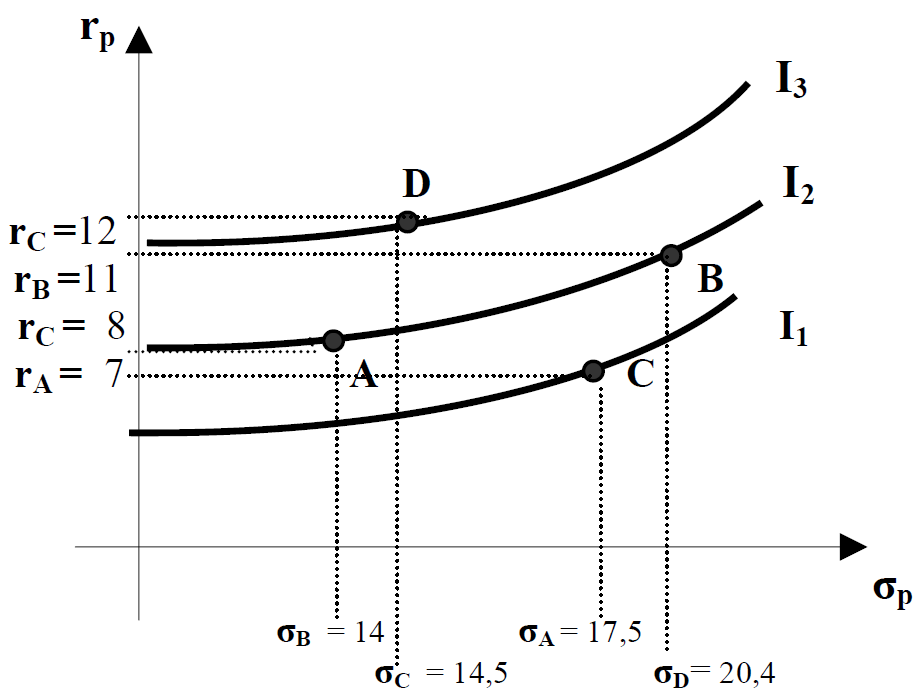
\includegraphics[width=10cm]{IC0.png}
\caption{Příklad indiferenčních křivek, zdroj: \cite{camsky} \label{obr_IC}}
\end{figure}
Na obrázku \ref{obr_IC} je očekávaná výnosnost portfolia, respektive směrodatná odchylka, označena $r_p$, respektive $\sigma_p$. Investorovi je jedno, zda investuje do portfolia $A$, či $B$, přestože mají různé očekávané výnosnosti a směrodatné odchylky. Investor je ochoten u~portfolia $B$ podstoupit vyšší riziko, avšak požaduje za to vyšší očekávanou výnosnost. Naopak u~portfolia $A$ je ochoten přijmout nižší očekávaný výnos výměnou za nižší riziko. Investor preferuje portfolia ležící na vyšších indiferenčních křivkách, neboť je schopen dosáhnout vyššího výnosu při stejném riziku, či naopak, stejného výnosu při nižším riziku. Např. portfolio $D$ ležící na $I_3$ je preferováno před portfoliem $A$ ležícím na $I_2$.  Tvar indiferenčních křivek je odvozen od axiomů \emph{nenasycenosti} a \emph{odporu k~riziku} \cite{camsky}.

Odpor k~riziku se u~jednotlivých investorů může značně lišit. V~důsledku toho mohou indifereční křivky nabývat různých podob. Vždy se však jedná o~konvexní rostoucí křivky, neboť s~rostoucím rizikem požaduje investor vyšší výnos. Indiferenční křivky pro různé typy investorů podle míry odporu k~riziku jsou znázorněny na obrázku \ref{obr_ICs}.
 
\begin{figure}[htb]
\centering
\subfigure[Investor s~vysokým odporem k~riziku]{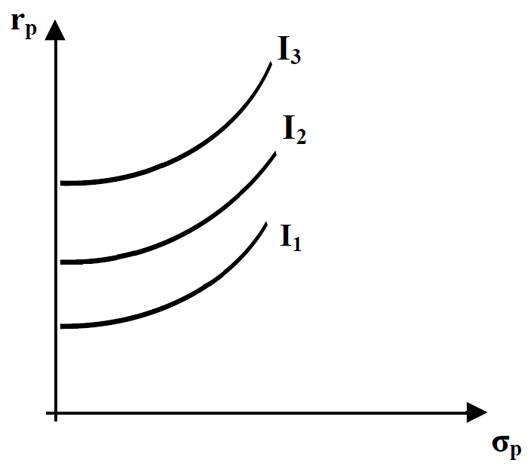
\includegraphics[width=7cm]{IC3.png}} 
\subfigure[Investor s~mírným odporem k~riziku]{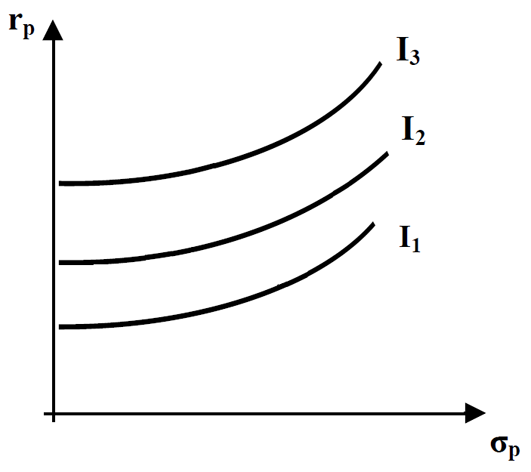
\includegraphics[width=7cm]{IC2.png}} 
\subfigure[Investor s~nepatrným odporem k~riziku]{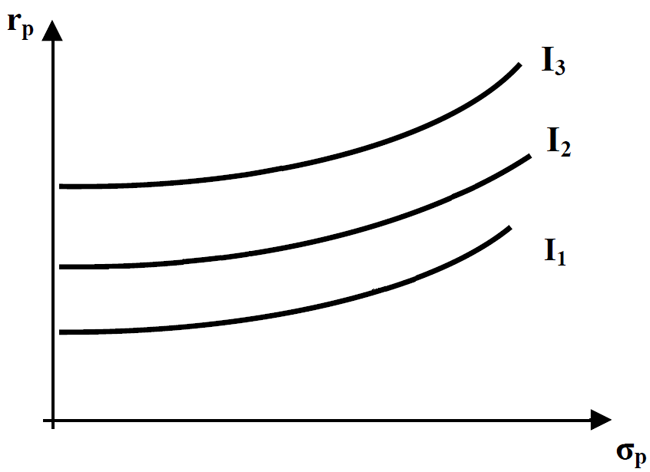
\includegraphics[width=8.5cm]{IC1.png}} 
\caption{Indiferenční křivky investora dle míry odporu k~riziku, zdroj: vlastní vyobrazení \label{obr_ICs}}
\end{figure}

\subsection{Efektivní množina}
Z~konečné množiny aktiv může investor poskládat nekonečně mnoho portfolií. Existuje totiž nekonečně mnoho $n$-tic reálných čísel $w_1,w_2,\dots,w_n$ splňujících podmínky \eqref{wr1} a \eqref{wr2}. Množinu všech portfolií složených z~aktiv $A_1,A_2,\dots,A_n$ nazýváme \emph{přípustná množina}. Přípustná množina je množinou všech dostupných portfolií. Při výběru portfolia se však investor může omezit pouze na podmnožinu všech portfolií, tzv. efektivní množinu.

\emph{Efektivní množina} je množina všech portfolií z~přípustné množiny, které splňují obě dvě následujících podmínky:
\begin{itemize}
\item v~přípustné množině neexistuje portfolio se stejným rizikem a vyšším očekávaným výnosem,
\item v~přípustné množině neexistuje portfolio se stejným očekávaným výnosem a nižším rizikem. 
\end{itemize}

Je zřejmě, že investor, který chce maximalizovat výnos a minimalizovat riziko, si nevybere žádné portfolio neležící v~efektivní množině. V~opačném případě, by totiž změnou portfolia mohl dosáhnout vyššího očekávaného výnosu při neměnném riziku, anebo stejného očekávaného výnosu při nižším riziku. Proto se při hledání optimálního portfolia stačí omezit právě na efektivní množinu.

\begin{figure}[htb]
\centering
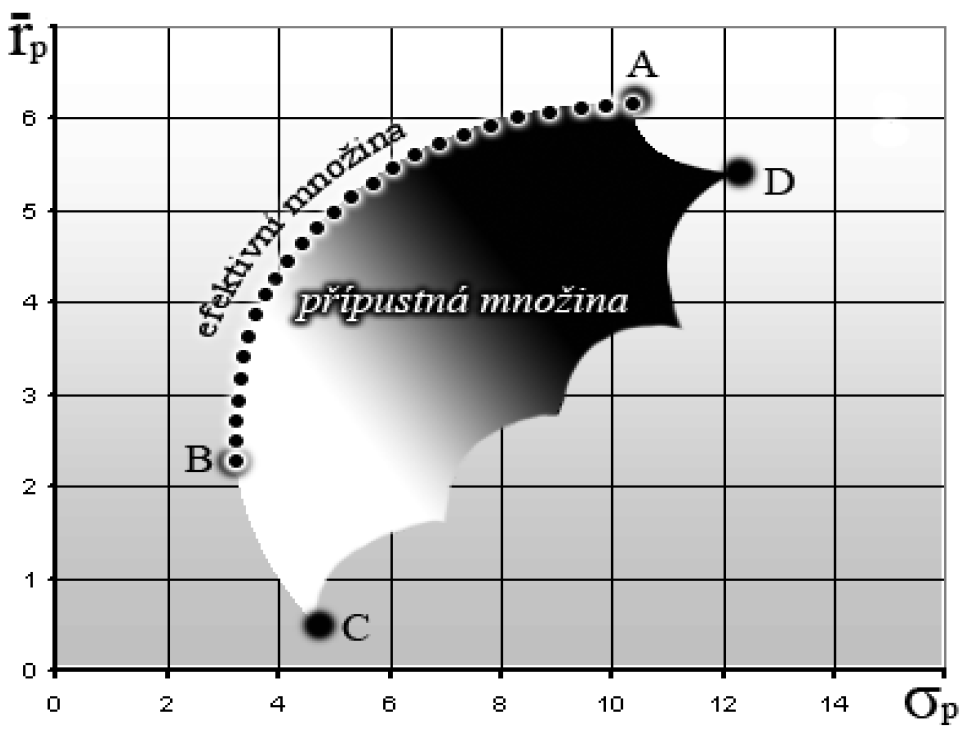
\includegraphics[width=10cm]{ef_mn.png}
\caption{Přípustná a efektivní množina, zdroj: \cite{camsky} \label{ef_mn}}
\end{figure}

Hledání efektivní množiny můžeme popsat následovně:
\begin{itemize}
\item pro každou fixní úroveň rizika nalezneme všechna dostupná portfolia s~maximální očekávanou výnosností, 
\item pro každou fixní úroveň očekávané výnosností nalezneme všechna dostupná portfolia s~minimálním rizikem,
\item do efektivní množiny zařadíme právě ta portfolia, která byla vybrána v~obou předchozích krocích.
\end{itemize}
Příklad přípustné a efektivní množiny je znázorněn na obrázku \ref{ef_mn}. Dle předchozího postupu bychom v~tomto případě hledali efektivní množinu následovně. Portfoliím s~maximální očekávanou výnosností při dané úrovni rizika odpovídají právě body ležící na hranici přípustné množiny mezi body $B$, $A$ a $A$,$D$. Portfoliím s~minimálním rizikem  při dané úrovni očekávané výnosnosti odpovídají právě body ležící na hranici přípustné množiny mezi body $C$, $B$ a $B$,$A$. Body spadající do obou těchto kategorií, tedy právě body ležící na hranici přípustné množiny mezi body $B$, $A$, tvoří efektivní množinu.

\subsection{Výběr optimálního portfolia}
V~předchozí části jsme ukázali, že investor si vybere portfolio z~efektivní množiny. Které konkrétní portfolio si vybere, však záleží na jeho preferencích. V~efektivní množině jsou portfolia s~různými očekávanými výnosnostmi a různými riziky. Investorův postoj k~riziku popisují indiferenční křivky. Zakreslíme-li tedy indiferenční křivky spolu s~efektivní množinou do jednoho obrázku, můžeme porovnat jednotlivá portfolia v~efektivní množině podle investorových preferencí.

\begin{figure}[htb]
\centering
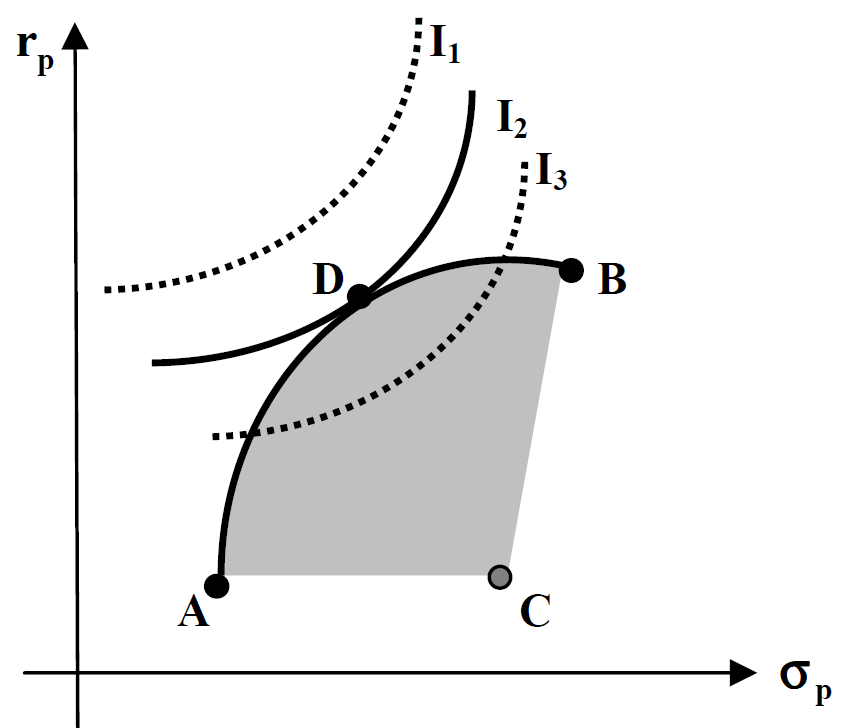
\includegraphics[width=10cm]{vyber.png}
\caption{Výběr optimálního portfolia, zdroj: \cite{camsky} \label{vyber}}
\end{figure}

Jak již víme, čím vyšší indiferenční křivka, na které portfolio leží, tím víc investor portfolio preferuje. Investor si proto vybere to portfolio z~efektivní množiny ležící na nejvyšší indiferenční křivce. Takovou křivkou je právě ta indiferenční křivka, která je tečnou efektivní množiny. Na obrázku \ref{vyber} se jedná o~indiferenční křivku $I_2$ a investor zvolí portfolio $D$.

\chapter{Praktická část}
  V této kapitole se budeme věnovat praktické aplikaci Markowitzovy teorie potrfolia. Jako nástroj ke zpracování dat poslouží rozšířený a několika chyb zbavený skript Travise Vaughta\cite{tvaught}. Je napsán v jazyce Python a využívá knihoven NumPy. Zdrojový kód původní verze je dostupný na internetu\cite{source}.
  
  Software je založen na Markowitzově teorii a k analýze aktiv historickou metodou používa metrik z CAPM. Samotný výpočet optima probíhá numerickou iterativní metodou převzatou z práce Williama Sharpa\cite{sharpe}.
  
  Zdrojem dat je Yahoo! Finance\cite{yahoo}. Byly použity výhradně akcie z indexu S\&P500, protože obsahuje známé a stabilní společnosti, do kterých je zároveň snadné investovat. Historický obdobím pro získání metrik je 1.1.2010 až 1.11.2011. Jako tolerance k risku pro finální optimalizaci byla zvolena poměrně nízká hodnota 0,05 ročně, která zajistí vyšší pestrost portfolia. Bezrizikové aktivum má nulový výnos a není povoleno obchodování na krátko.
  \section{Hardware}
    Toto portfolio obsahuje významné výrobce počítačového hardware. Z tabulek je patrno, že největšího ročního výnosu dosahuje Apple Inc. a nejnižšího rizika IBM, přičemž si stále zachovává slušný růst. Optimalizované portfolio obsahuje právě tyto dvě akcie a dále ještě nepatrný podíl Intel Corporation. Jeho volatilita je 0.193, což je méně než obě hlavní akcie. Roční výnos dosahuje 24.37\%, tedy více než má samostatně nejméně riziková akcie.
    \begin{table}[htb]
      \centering
      \begin{tabular}{|l|l|r|r|}
        \hline
        Symbol&Název&Volatilita&Roční výnos\\\hline\hline
        A&Agilent Technologies &0.402&16.43\%\\\hline
        AAPL&Apple Inc. &0.266&37.57\%\\\hline
        AMD&Advanced Micro Devices &0.497&-16.46\%\\\hline
        DELL&Dell Inc. &0.345&9.585\%\\\hline
        HPQ&Hewlett-Packard &0.334&-31.4\%\\\hline
        IBM&International Bus. Machines &0.198&20.96\%\\\hline
        INTC&Intel Corp. &0.254&14.2\%\\\hline
        NVDA&Nvidia Corporation &0.512&-0.09651\%\\\hline
        TXN&Texas Instruments &0.267&13.72\%\\\hline
      \end{tabular}
      \caption{Akcie pro porfolio hardware}
    \end{table}

    \begin{figure}[htb]
      \centering
      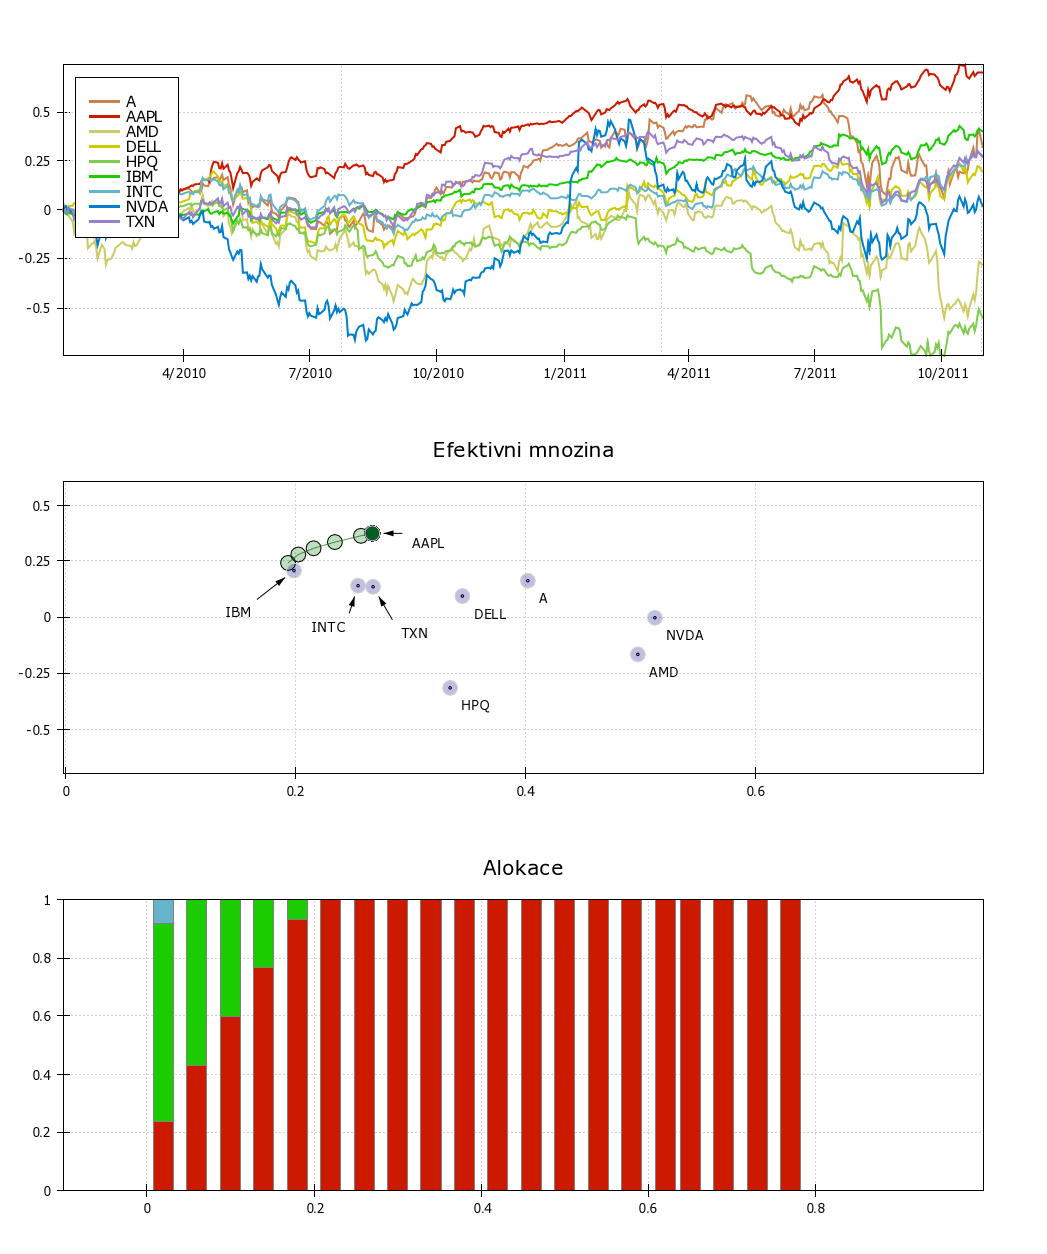
\includegraphics[height=0.90\textheight]{hw1.png}
      \caption{Grafické zobrazení portfolia hardware}
    \end{figure}

    \begin{table}[htb]
      \centering
      \begin{tabular}{|l|l|r|}
        \hline
        Symbol&Název&Alokace\\\hline\hline
        AAPL&Apple Inc. &0.346\\\hline
        IBM&International Bus. Machines &0.648\\\hline
        INTC&Intel Corp. &0.0069\\\hline
      \end{tabular}
      \caption{Optimální portfolio hardware}
    \end{table}
    
  \clearpage
  \section{Software a internetové služby}
    Zde se zabýváme velkými softwarovými firmami a poskytovateli elektronických služeb. Z metrik je vidět, že tyto akcie dosahují nemalých zhodnocení, ovšem často za cenu vysoké volatility. Optimalizované portfolio má nízký roční výnos 3,736\% a poměrně vysokou volatilitu 0.218, která je ovšem menší než u jakékoliv jednotlivé akcie ze sektoru. Je to způsobeno tím, že akcie firmy Microsoft má záporný roční výnos -4.513\%, ale přesto tvoří více než polovinu potfolia, neboť je vnímána jako konkurent k v podstatě všem ostatním, což způsobuje silnou zápornou korelaci. 
    \begin{table}[htb]
      \centering
      \begin{tabular}{|l|l|r|r|}
        \hline
        Symbol&Název&Volatilita&Roční výnos\\\hline\hline
        ADBE&Adobe Systems &0.356&-7.255\%\\\hline
        ADSK&Autodesk Inc. &0.397&23.36\%\\\hline
        AKAM&Akamai Technologies Inc &0.478&12.77\%\\\hline
        EBAY&eBay Inc. &0.35&20.87\%\\\hline
        ERTS&Electronic Arts &0.362&19.38\%\\\hline
        GOOG&Google Inc. &0.291&0.1524\%\\\hline
        MSFT&Microsoft Corp. &0.226&-4.513\%\\\hline
        ORCL&Oracle Corp. &0.287&19.16\%\\\hline
        SYMC&Symantec Corp. &0.306&-0.5626\%\\\hline
        YHOO&Yahoo Inc. &0.351&0.2939\%\\\hline
      \end{tabular}
      \caption{Akcie pro porfolio software}
    \end{table}

    \begin{figure}[htb]
      \centering
        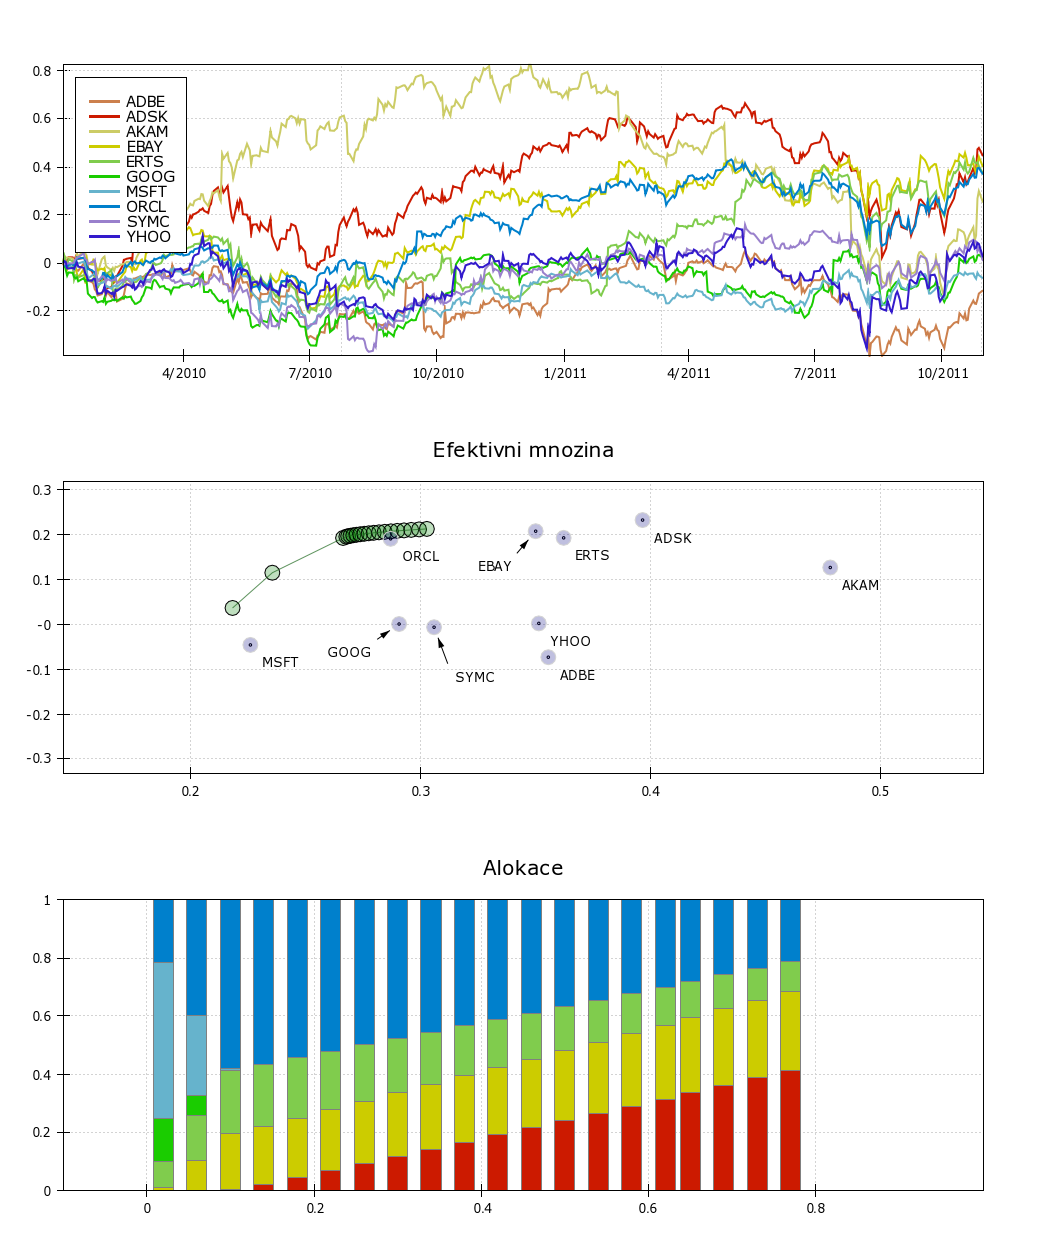
\includegraphics[height=0.90\textheight]{sw1.png}
       \caption{Grafické zobrazení portfolia software}
    \end{figure}

    \begin{table}[htb]
      \centering
      \begin{tabular}{|l|l|r|}
        \hline
        Symbol&Název&Alokace\\\hline\hline
        EBAY&eBay Inc. &0.0129\\\hline
        ERTS&Electronic Arts &0.0888\\\hline
        GOOG&Google Inc. &0.149\\\hline
        MSFT&Microsoft Corp. &0.534\\\hline
        ORCL&Oracle Corp. &0.216\\\hline
      \end{tabular}
      \caption{Optimální portfolio software}
    \end{table}

  \clearpage
  \section{Výrobci farmaceutik}
    Dalším sektorem jsou výrobci farmaceutik. Z tabulek ihned vidíme, že všechny akcie mají v podstatě stejný charakter -- nízký výnos i volatilitu. Přesto se optimalizací podařilo dosáhnout volatility 0.137, což je méně než má kterákoliv akcie. Výnos 3.359\% je přibližně aritmetický průměr výnosů v sektoru.
    
    \begin{table}[htb]
      \centering
      \begin{tabular}{|l|l|r|r|}
        \hline
        Symbol&Název&Volatilita&Roční výnos\\\hline\hline
        ABT&Abbott Labs &0.16&3.525\%\\\hline
        BAX&Baxter International Inc. &0.244&1.14\%\\\hline
        JNJ&Johnson \& Johnson &0.15&3.236\%\\\hline
        MRK&Merck \& Co. &0.213&1.664\%\\\hline
        PFE&Pfizer Inc. &0.226&6.494\%\\\hline
      \end{tabular}
      \caption{Akcie pro porfolio farmaceutik}
    \end{table}

    \begin{figure}[htb]
      \centering
        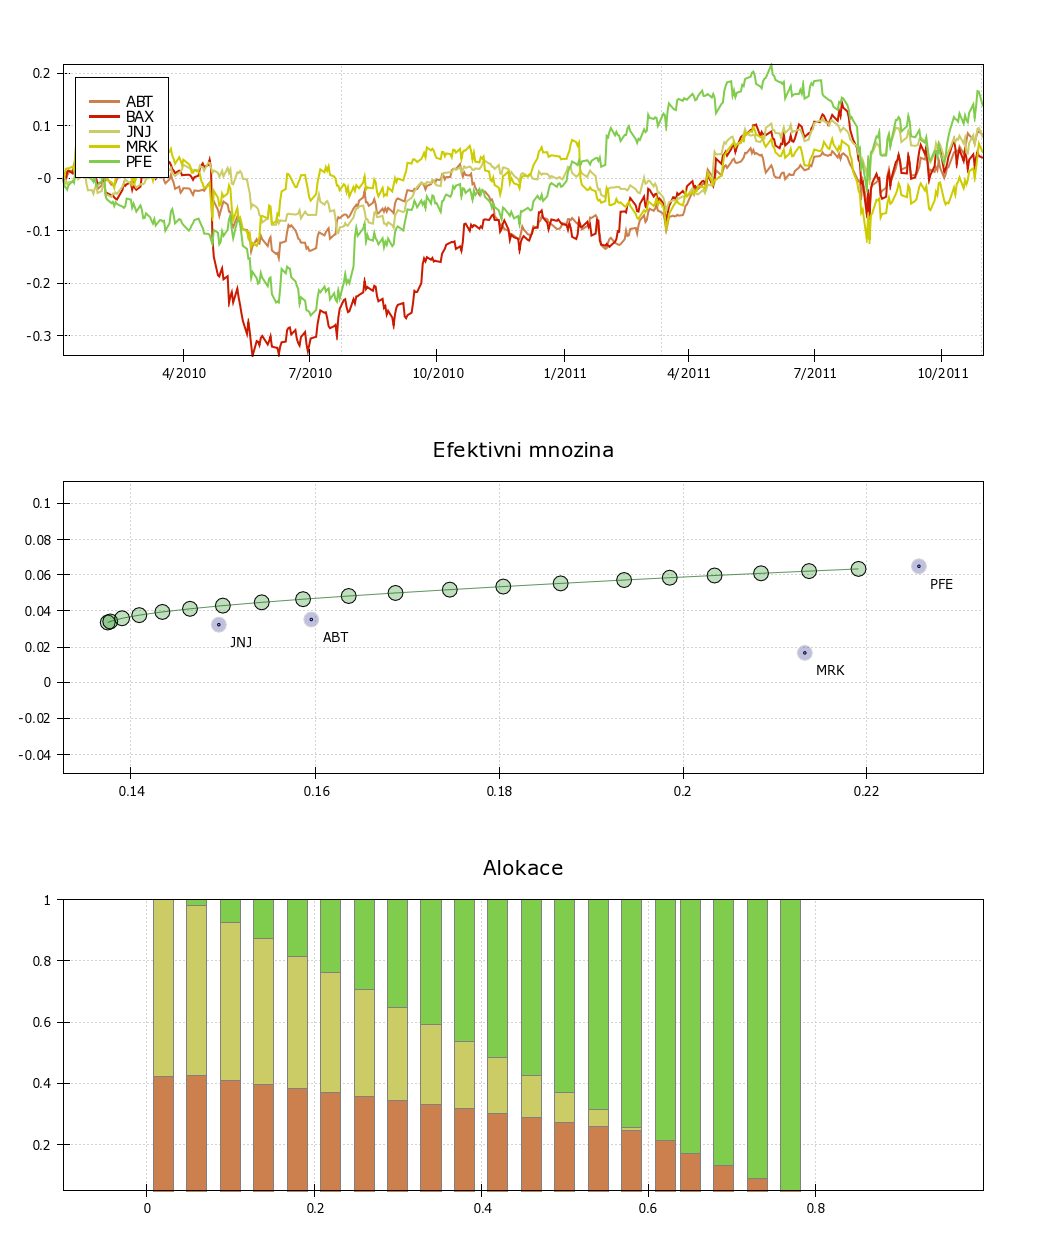
\includegraphics[height=0.90\textheight]{drugs1.png}
       \caption{Grafické zobrazení portfolia farmaceutik}
    \end{figure}

    \begin{table}[htb]
      \centering
      \begin{tabular}{|l|l|r|}
        \hline
        Symbol&Název&Alokace\\\hline\hline
        ABT&Abbott Labs &0.424\\\hline
        JNJ&Johnson \& Johnson &0.576\\\hline
      \end{tabular}
      \caption{Optimální portfolio farmaceutik}
    \end{table}
    
  \clearpage
  \section{Finanční sektor}
    Sektor financí obsahuje velmi rozličné akciové tituly. Výnosy se pohybují od -34\% do +17\%. Společná je však velmi vysoká volatilita. Optimalizací se ji podřilo dramaticky snížít na 0.286 při zachování přijatelného výnosu 9.456\%. Zde akcie Goldman Sachs působí přes výraznou ztrátu jako stabilizátor.
    
    \begin{table}[htb]
      \centering
      \begin{tabular}{|l|l|r|r|}
        \hline
        Symbol&Název&Volatilita&Roční výnos\\\hline\hline
        AXP&American Express &0.315&17.55\%\\\hline
        BAC&Bank of America Corp. &0.479&-34.62\%\\\hline
        C&Citigroup Inc. &0.445&5.03\%\\\hline
        GS&Goldman Sachs Group &0.331&-19.59\%\\\hline
        JPM&JPMorgan Chase \& Co. &0.343&-5.188\%\\\hline
        MS&Morgan Stanley &0.457&-20.4\%\\\hline
        NDAQ&NASDAQ OMX Group &0.352&16.9\%\\\hline
        NYX&NYSE Euronext &0.398&12.58\%\\\hline
      \end{tabular}
      \caption{Akcie pro porfolio financí}
    \end{table}

    \begin{figure}[htb]
      \centering
        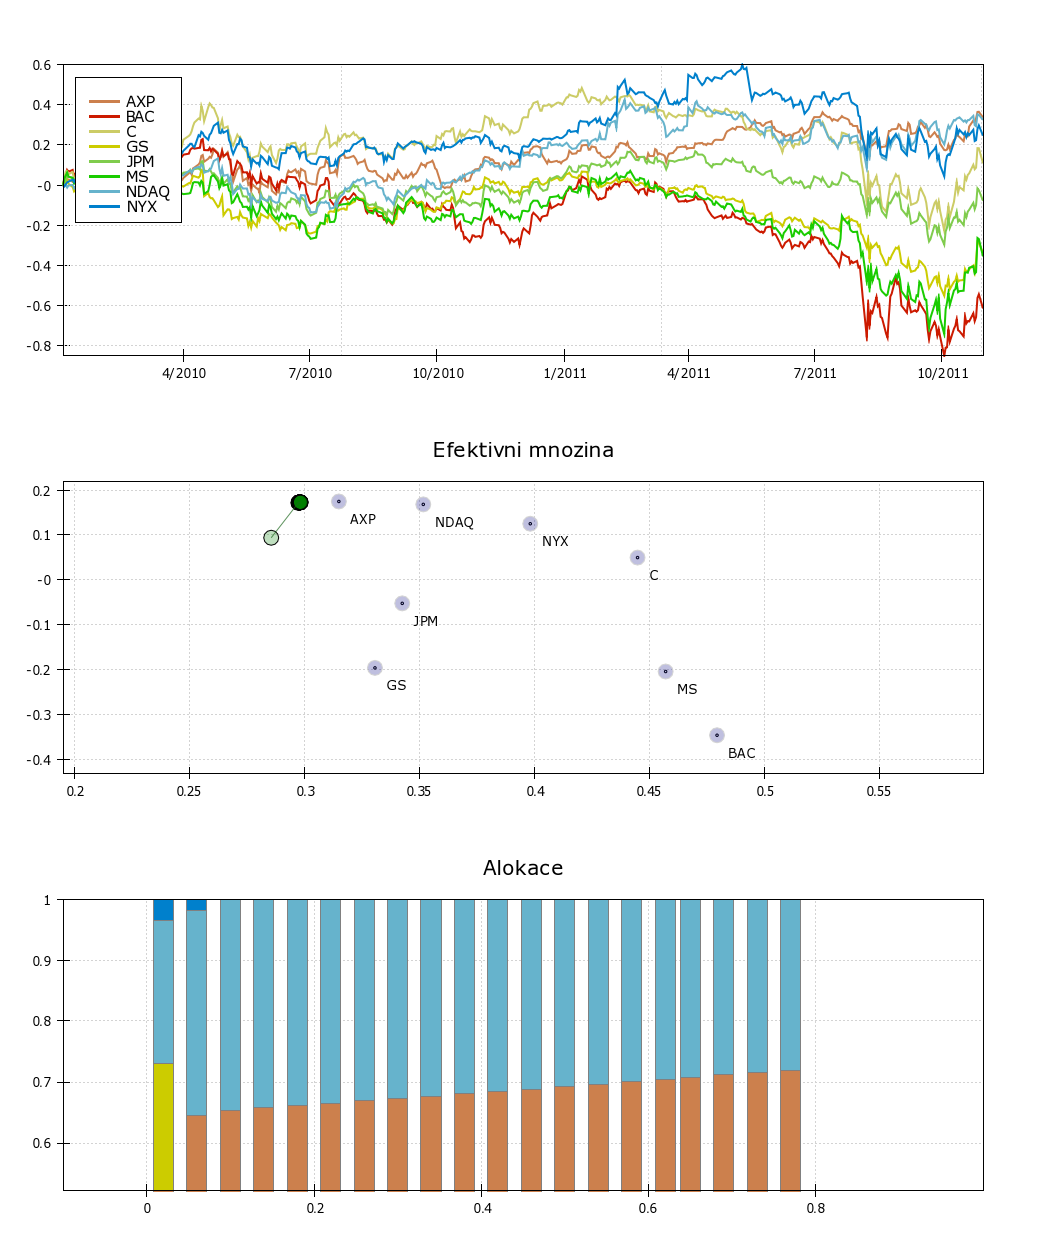
\includegraphics[height=0.90\textheight]{fin1.png}
       \caption{Grafické zobrazení portfolia financí}
    \end{figure}

    \begin{table}[htb]
      \centering
      \begin{tabular}{|l|l|r|}
        \hline
        Symbol&Název&Alokace\\\hline\hline
        AXP&American Express &0.522\\\hline
        GS&Goldman Sachs Group &0.209\\\hline
        NDAQ&NASDAQ OMX Group &0.235\\\hline
        NYX&NYSE Euronext &0.0341\\\hline
      \end{tabular}
      \caption{Optimální portfolio financí}
    \end{table}
    
  \clearpage
  \section{Průmysl}
    V sektoru průmyslu vidíme až na společnost 3M solidní výnosnost za přiměřené volatility. Caterpillar dosahuje ročního zhodnocení dokonce přes 33\%. V našem optimalizovaném nízkorizikové portfoliu se přesto neobjevuje, protože je příliš silně pozitivně korelován s ostatními. Dosahujeme nižšího výnosu 6.073\% a stejně tak volatility 0.236 z toho důvodu, že přes 60\%  portfolia tovří 3M.
    
    \begin{table}[htb]
      \centering
      \begin{tabular}{|l|l|r|r|}
        \hline
        Symbol&Název&Volatilita&Roční výnos\\\hline\hline
        BA&Boeing Company &0.299&14.5\%\\\hline
        CAT&Caterpillar Inc. &0.34&33.5\%\\\hline
        GE&General Electric &0.286&10.3\%\\\hline
        HON&Honeywell Int'l Inc. &0.29&20.14\%\\\hline
        MMM&3M Company &0.24&1.624\%\\\hline
      \end{tabular}
      \caption{Akcie pro porfolio průmyslu}
    \end{table}

    \begin{figure}[htb]
      \centering
        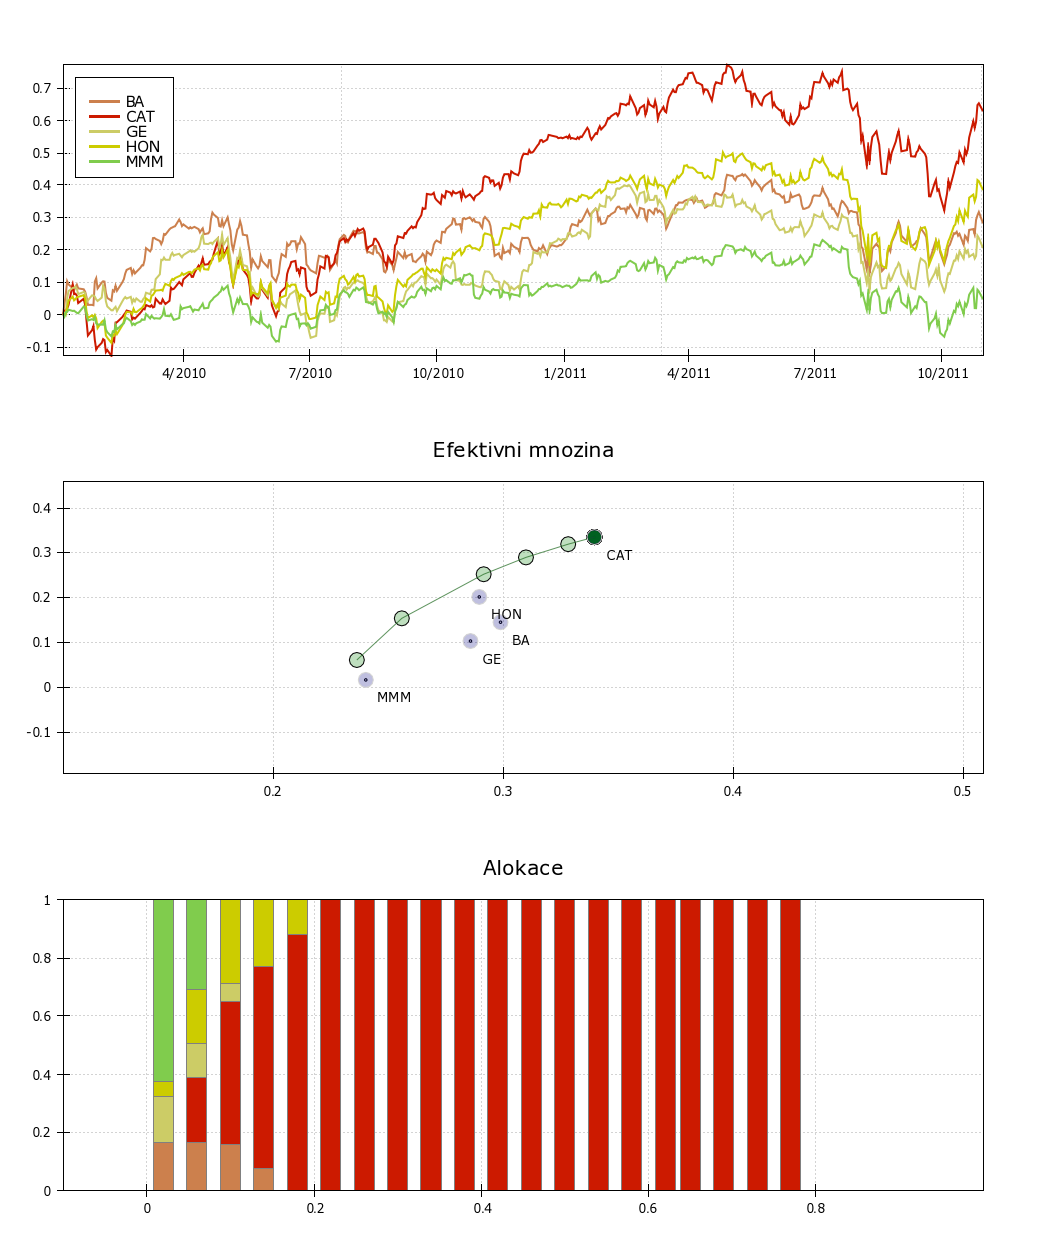
\includegraphics[height=0.90\textheight]{ind1.png}
       \caption{Grafické zobrazení portfolia průmyslu}
    \end{figure}

    \begin{table}[htb]
      \centering
      \begin{tabular}{|l|l|r|}
        \hline
        Symbol&Název&Alokace\\\hline\hline
        BA&Boeing Company &0.165\\\hline
        GE&General Electric &0.16\\\hline
        HON&Honeywell Int'l Inc. &0.0501\\\hline
        MMM&3M Company &0.624\\\hline
      \end{tabular}
      \caption{Optimální portfolio průmyslu}
    \end{table}
    
  \clearpage
  \section{Nejcennější značky}
    Zde budeme zkoumat akcie majitelů 10 nejcennějších značek podle Financial Times\cite{ft}, které jsou obsaženy v S\&P500. Snad až na Altria Group, která je majitelem značky Marlboro, jsou všechny jasné. Jsou zde obsaženy tituly sektorů IT, komunikací, průmyslu i konzumního zboží. Díky této diverzitě bylo dosaženo nízké volatility 0.136 a vysokého výnosu 24.24\%.   
    \begin{table}[htb]
      \centering
      \begin{tabular}{|l|l|r|r|}
        \hline
        Symbol&Název&Volatilita&Roční výnos\\\hline\hline
        AAPL&Apple Inc. &0.266&37.57\%\\\hline
        GE&General Electric &0.286&10.3\%\\\hline
        GOOG&Google Inc. &0.291&0.1524\%\\\hline
        IBM&International Bus. Machines &0.198&20.96\%\\\hline
        KO&Coca Cola Co. &0.164&13.13\%\\\hline
        MCD&McDonald's Corp. &0.161&24.78\%\\\hline
        MO&Altria Group Inc. &0.157&24.47\%\\\hline
        MSFT&Microsoft Corp. &0.226&-4.513\%\\\hline
        T&AT\&T Inc. &0.166&8.371\%\\\hline
        VZ&Verizon Communications &0.18&12.74\%\\\hline
      \end{tabular}
      \caption{Akcie pro porfolio značek}
    \end{table}

    \begin{figure}[htb]
      \centering
        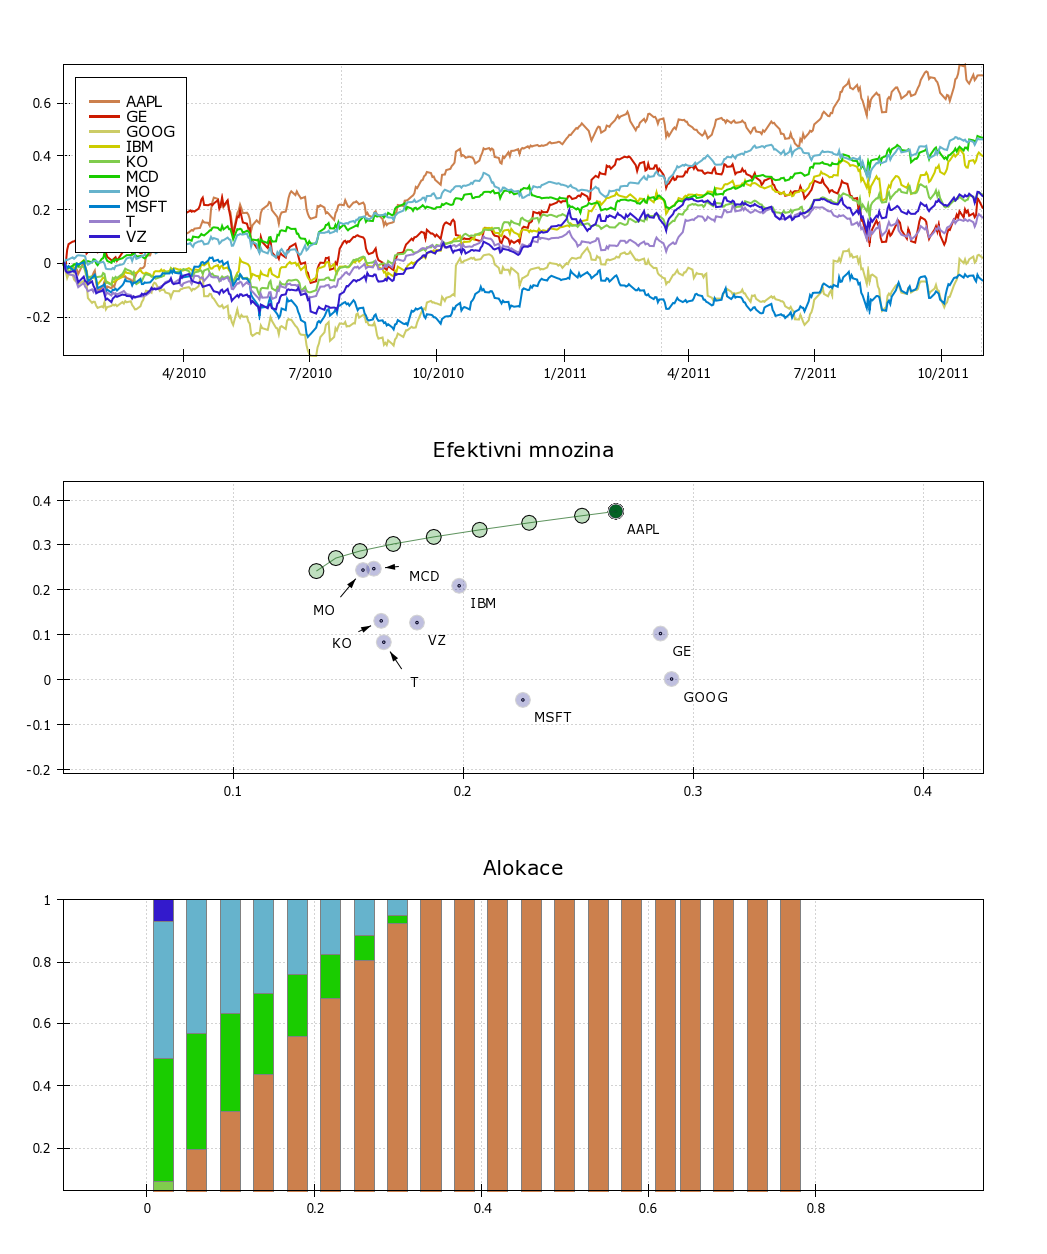
\includegraphics[height=0.90\textheight]{brands1.png}
       \caption{Grafické zobrazení portfolia značek}
    \end{figure}

    \begin{table}[htb]
      \centering
      \begin{tabular}{|l|l|r|}
        \hline
        Symbol&Název&Alokace\\\hline\hline
        AAPL&Apple Inc. &0.0617\\\hline
        KO&Coca Cola Co. &0.0311\\\hline
        MCD&McDonald's Corp. &0.394\\\hline
        MO&Altria Group Inc. &0.444\\\hline
        VZ&Verizon Communications &0.0688\\\hline
      \end{tabular}
      \caption{Optimální portfolio značek}
    \end{table}
    
  \clearpage
  \section{Deset nejziskovějších titulů}
    Tento seznam nejziskovějších titulů byl získán výpočtem příslušných metrik pro všechny akcie S\&P500. Opět vidíme společnosti ze všech oblastí hospodářství. Optimalizací bylo získáno portfolio s volatilitou 0.214 a vysokým výnosem 46.52\%, na který se ovšem vzhledem k použití čistě historické metody nelze do budoucna spolehnout.
    \begin{table}[htb]
      \centering
      \begin{tabular}{|l|l|r|r|}
        \hline
        Symbol&Název&Volatilita&Roční výnos\\\hline\hline
        ACAS&American Capital Strategies Ltd &0.502&72.66\%\\\hline
        AN&AutoNation Inc. &0.352&43.83\%\\\hline
        ANF&Abercrombie \& Fitch Co. &0.457&52.22\%\\\hline
        BIIB&BIOGEN IDEC Inc. &0.303&46.06\%\\\hline
        CMI&Cummins Inc. &0.417&50.12\%\\\hline
        EL&Estee Lauder Cos. &0.317&43.38\%\\\hline
        EP&El Paso Corp. &0.39&55.31\%\\\hline
        FDO&Family Dollar Stores &0.302&46.62\%\\\hline
        LTD&Limited Brands Inc. &0.346&50.85\%\\\hline
        MBI&MBIA Inc. &0.644&60.09\%\\\hline
      \end{tabular}
      \caption{Akcie pro porfolio Top10}
    \end{table}

    \begin{figure}[htb]
      \centering
        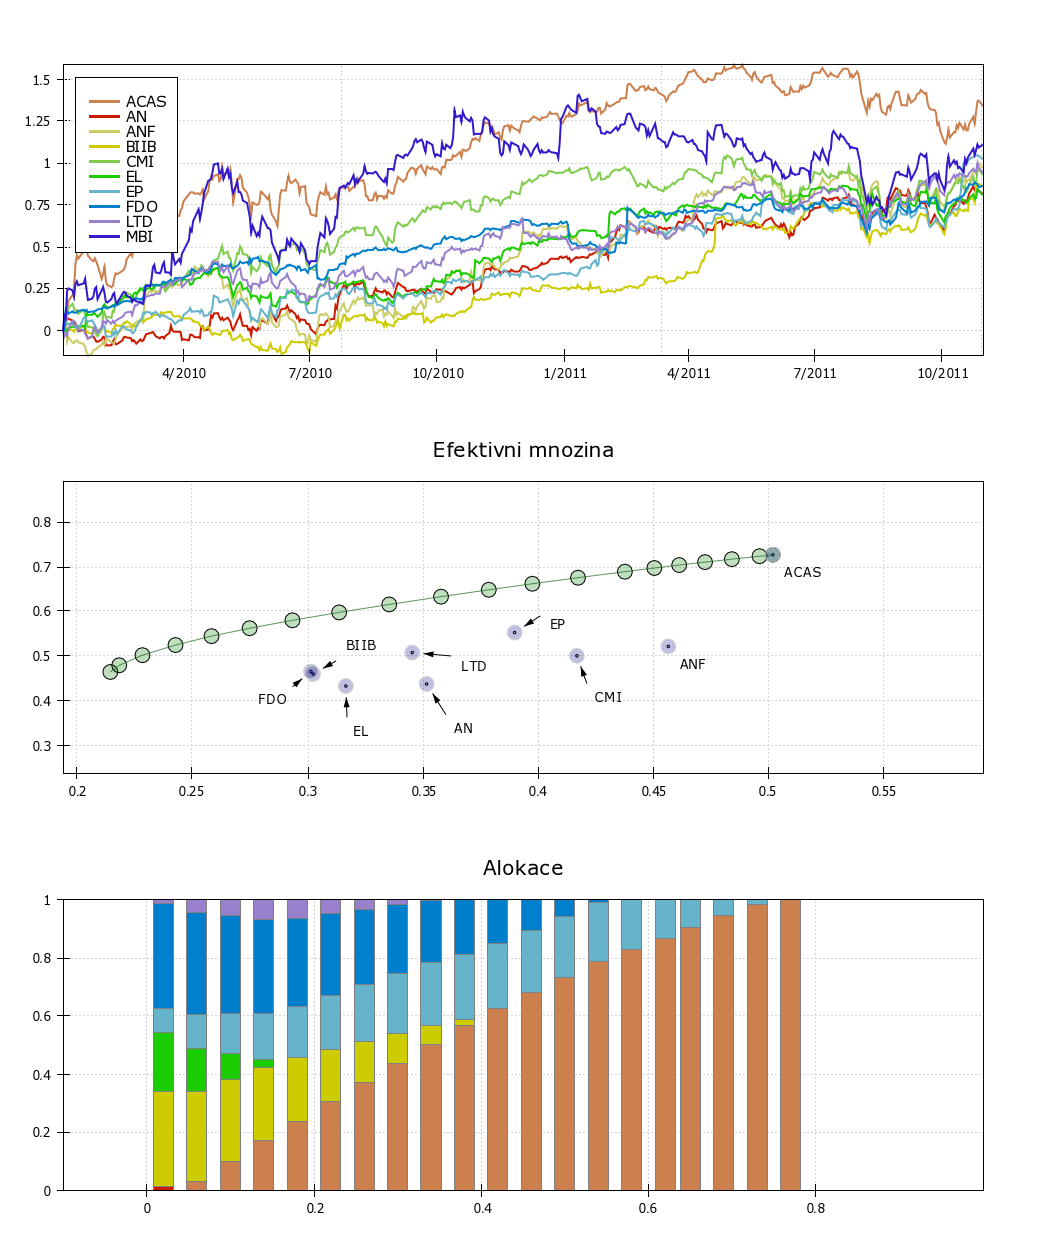
\includegraphics[height=0.90\textheight]{top10.png}
       \caption{Grafické zobrazení portfolia Top10}
    \end{figure}

    \begin{table}[htb]
      \centering
      \begin{tabular}{|l|l|r|}
        \hline
        Symbol&Název&Alokace\\\hline\hline
        AN&AutoNation Inc. &0.0163\\\hline
        BIIB&BIOGEN IDEC Inc. &0.326\\\hline
        EL&Estee Lauder Cos. &0.201\\\hline
        EP&El Paso Corp. &0.0828\\\hline
        FDO&Family Dollar Stores &0.36\\\hline
        LTD&Limited Brands Inc. &0.014\\\hline

      \end{tabular}
      \caption{Optimální portfolio Top10}
    \end{table}

  \clearpage
  \section{Celý S\&P500}
    Zde byl algoritmus spuštěn na všechny akcie z S\&P500, které nevykazovaly při zpracování chybu. Výsledkem je následující portfolio s volatilitou 0.119 a výnosem 30.32\%.

    \begin{table}[htb]
      \centering
      \begin{tabular}{|l|l|r|r|r|}
        \hline
        Symbol&Název&Alokace&Volatilita&Roční výnos\\\hline\hline
        AZO&AutoZone Inc. &0.287&0.177&39.94\%\\\hline
        BIIB&BIOGEN IDEC Inc. &0.0446&0.303&46.06\%\\\hline
        FDO&Family Dollar Stores &0.0744&0.302&46.62\%\\\hline
        HSY&The Hershey Company &0.127&0.198&28.72\%\\\hline
        MCD&McDonald's Corp. &0.0317&0.161&24.78\%\\\hline
        MO&Altria Group Inc. &0.105&0.157&24.47\%\\\hline
        NEM&Newmont Mining Corp. (Hldg. Co.) &0.0161&0.3&22.29\%\\\hline
        SO&Southern Co. &0.315&0.129&19.01\%\\\hline
      \end{tabular}
      \caption{Optimální portfolio S\&P500}
    \end{table}

\renewcommand{\bibname}{Seznam použité literatury}
\begin{thebibliography}{9}
\addcontentsline{toc}{chapter}{Seznam použité literatury}
\thispagestyle{plain}
\bibitem{camsky} ČÁMSKÝ, František. \emph{Teorie portfolia.} 2. přeprac. a rozš. vyd. Brno : Masarykova univerzita, 2007. 115 s. ISBN 9788021042520.
\bibitem{markowitz} MARKOWITZ, Harry. \emph{Portfolio Selection.} The Journal of Finance. Mar., 1952, Vol. 7, No. 1, s. 77-91. 

\bibitem{tvaught}
VAUGHT, Travis. Travis Vaught Blog [online]. 2011-09-01 [cit. 2011-11-26]. Modern Portfolio Theory - A Python Implementation. Dostupné z WWW: \url{http://travisvaught.blogspot.com/2011/09/modern-portfolio-theory-python.html}.

\bibitem{source}
VAUGHT, Travis. GitHub [online]. 2009-10-31 [cit. 2011-11-26]. Portfolio metrics. Dostupné z WWW: \url{https://github.com/tvaught/experimental/tree/master/portfolio_metrics}.

\bibitem{sharpe}
SHARPE, William F., William F. Shapre personal page [online]. 2008 [cit. 2011-11-26]. The Gradient Method. Dostupné z WWW: \url{http://www.stanford.edu/~wfsharpe/mia/opt/mia_opt1.htm}.

\bibitem{yahoo}
Yahoo! Inc. Yahoo! Finance [online]. c2011 [cit. 2011-11-26]. Dostupné z WWW: \url{http://finance.yahoo.com/}.

\bibitem{ft}
Finacial Times. Financial Times Special Report [online]. 2011-05-19 [cit. 2011-11-26]. Global Brands. Dostupné z WWW: \url{http://www.millwardbrown.com/Libraries/Optimor_BrandZ_Files/2011_BrandZ_FinancialTimes_SpecialReport.sflb.ashx}.
\end{thebibliography}
\end{document}
